% ------------------------------------------------------------------------------
% Mathematics Project Report Template
% by Jon Shiach 2019
% Manchester Metropolitan University
% ------------------------------------------------------------------------------
\documentclass[11pt]{report} 

\usepackage{projectreport}

% Define 'keyword' environment if not using elsarticle
\newenvironment{keyword}{\par\noindent\textbf{Keywords:} }{\par}


% ------------------------------------------------------------------------------
% Enter your details here
% ------------------------------------------------------------------------------
\newcommand{\name}{Celumusa H Zulu}
\newcommand{\degree}{Master of Commerce}
\newcommand{\programme}{Information Technology Management}
\newcommand{\projecttitle}{The role of IT leadership in realizing the return on investment of AI coding assistants.} % Research project title as approved by the CBE HDC (case sensitive)
\newcommand{\supervisor}{Dr. Siyabonga Mhlongo}
\newcommand{\submissionyear}{2026}

% ------------------------------------------------------------------------------
% Document
% ------------------------------------------------------------------------------
\begin{document}
	
\maketitle

% ------------------------------------------------------------------------------
% Top matter
% ------------------------------------------------------------------------------
\chapter*{Abstract}
\addcontentsline{toc}{chapter}{Abstract}
\blindtext[1]

% ------------------------------------------------------------------------------
% Background
% ------------------------------------------------------------------------------
\chapter*{Background}
\addcontentsline{toc}{chapter}{Abstract}
Artificial intelligence (AI) is one of the important structural influencers on productivity growth and competitive advantage today \autocite{Gillespie2025}. As of 2023, generative AI systems have progressed from experimentation to operationalization within organizational processes \autocite{Gillespie2025}. Recent global studies suggest that organizations are investing more in AI with clear expectations of understanding tangible economic gains, cost savings, and performance improvements \autocite{Gillespie2025}. Research on information systems and management has advanced from adoption to value understanding, with a focus on distinguishing organizational value from investment in AI technologies as a function of organizational governance and management capability rather than technological capability \autocite{Hossain2025}.

In software engineering, generative AI tools represent one of the most prominent manifestations of AI-enabled augmentation \autocite{Peng2023}. Providing developers with functionalities such as code suggestions and entire code functions in real time based on context, documentation, and debugging \autocite{Peng2023}.Practical controlled experiments provide conclusive evidence that AI-assisted developers complete software development tasks faster and report increased productivity of about 55.8\% compared with control groups \autocite{Peng2023}. Collaboration between humans and AI systems is a paradigm shift from the traditional concept of automation, in which AI enhances developers' capabilities rather than replacing them with machines \autocite{Peng2023}. Initial performance improvements demonstrated in controlled promising experiments may not necessarily guarantee long-term organizational performance benefits. Empirical studies report considerable variation in the productivity gains from AI-assisted software development tasks across software development teams and organizations.

Both organizational culture and leadership have traditionally been acknowledged as factors that impact the success of technology implementation. In the digital domain, it is the values and norms that foster a culture of experimentation, learning, and data-driven decision-making, as well as a willingness to adopt technological changes. New studies have found that digital culture reinforces the association between human AI competencies and innovation outcomes, suggesting that cultural readiness moderates the performance effects of AI investments \autocite{An2024}. Likewise, the same is true for employee engagement in AI initiatives, ethical governance, and leadership's role in influencing strategic alignment. While the importance of digital culture and leadership is increasingly acknowledged in the AI adoption domain, the current body of research remains dispersed \autocite{An2024}. Most studies analyse AI adoption from a macro-organizational perspective or focus on individual productivity effects, failing to consider the integration of digital culture, leadership, and ROI in software engineering \autocite{Peng2023}. ROI is increasingly becoming the sole rationale for investing in enterprise AI initiatives.

African organizations are accelerating the adoption of AI technologies to address structural inefficiencies and resource limitations. Emerging market organizations have reported high levels of workplace AI experimentation and positive attitudes toward AI productivity \autocite{Gillespie2025}. However, the extant literature also emphasizes the lack of digital skills pipelines, governance maturity, and leadership ability, among other things, as difficulties associated with the adoption of GenAI technologies \autocite{Hughes2026}. In this regard, the importance of organizational culture and leadership cannot be overstated. In the absence of strategic direction, trust, and a learning-oriented culture, the adoption of AI technologies is more inclined toward fragmentation and symbolic adoption than toward creating value. The digital transformation landscape in Africa is a valid environment for exploring the impact of socio-organizational factors on the achievement of returns from AI technologies.

In the context of software engineering in South Africa, it provides a relevant setting for understanding how organizations embrace and use advanced AI tools. Research indicates that AI is emerging as a key factor influencing organizational change and shaping work practices and culture as organizations increasingly embrace AI tools across their business processes and operations \autocite{Murire2024}. There are opportunities and challenges to address to leverage organizational performance through AI adoption and alignment with organizational culture and structure, as indicated by research reviews on AI tool adoption in organizations \autocite{Romeo2025}. Though the adoption of AI technology affects many aspects of the organization's performance positively, like productivity and output, the effect of AI technology on aspects like the organization's culture and employees' morale and engagement is complicated and depends on many factors, as indicated by the study on the impact of AI tools in workplace settings \autocite{Kassa2025}. Studies on the effect of generative AI tools on software engineering have indicated that AI technology positively affects organizations by enhancing productivity in coding and other software engineering activities through employees' adoption of AI tools \autocite{Alenezi2025}.

Leadership and organizational culture play an important role in the interpretation, adoption, and usage of AI technologies by work teams. Research on AI adoption has found that AI-related technology adoption is also dependent on leadership styles that facilitate embedding technology initiatives into organizational culture \autocite{Romeo2025}. Research on the adoption of AI-related technology has also found that the adoption of AI-related technology is dependent on the adoption of the organizational culture that is conducive to the adoption of the technology \autocite{Kassa2025}. Organizational culture research further indicates that cultural factors, specifically norms related to innovation, collaboration, and adaptability, modulate how employees engage with AI tools and integrate them into their work \autocite{Murire2024}. In software engineering teams, where AI coding assistants alter routines and task assignments, leadership and culture therefore likely determine the extent to which AI investments yield returns in productivity, quality, and financial outcomes, making them essential variables in understanding realized returns on investment.

% ------------------------------------------------------------------------------
% Problem Statement
% ------------------------------------------------------------------------------
\chapter*{Problem Statement}
\addcontentsline{toc}{chapter}{Problem Statement}
Generative AI has shifted its focus from experiment deployment to integrating it into the core knowledge work process. Substantial experimental results show that generative AI can significantly improve the productivity and quality of cognitive work outcomes, especially among lower-performing members, thereby affecting the performance distribution within the organization \autocite{Noy2023}. Field experiment results show that the application of generative AI in the real world can improve the organization's productivity and influence relevant outcomes, such as task completion and retention, indicating that the ROI on generative AI comes from its application within the organization, not the technology itself \autocite{Brynjolfsson2025}. In the software development field, three large-scale field experiments have shown that providing developers with GitHub Copilot can improve task completion and development activities, providing empirical support for the ROI of generative AI in coding assistance \autocite{Cui2026}. Controlled experiment results show that developers using AI coding assistance complete programming tasks more quickly and at a higher rate, providing a business case for AI coding assistance tools based on productivity \autocite{Peng2023}.

Despite these measurable improvements, existing research evidence consistently shows that the performance impact differs across contexts. Research in software engineering has shown that AI-assisted code generation produced by GitHub Copilot improves speed but also creates variability in correctness, maintainability, and review effort; this shows the value to depend on the management and integration of such tools and systems \autocite{MoradiDakhel2023}. Research on AI governance in organizations has argued that to sustain value, organizations must have structured processes and systems to ensure clear accountability and supervisory leadership to transform experimentation into sustained performance improvement \autocite{Maentymaeki2022}. Research on organizational innovation with generative AI has also shown that organizations can obtain different performance impacts depending on whether AI is used for automation or augmentation; this shows the role of strategic leadership and organizational culture in determining the benefits obtained \autocite{Holmstroem2025}. Overall, this existing research evidence shows the role of organizational culture and strategic leadership in determining whether the improvements in productivity due to AI coding assistants can be sustained and converted to measurable return on investment.

The relevance of these mechanisms can be further accentuated in the context of Africa since organizations face structural limitations in skills development, governance, and digital sophistication. An empirical study of AI readiness in Africa identified the level of preparedness and the institutional ability to adopt AI, thus emphasizing the role of organizations in the transition from AI pilot projects to performance results \autocite{Isagah2024}. In the context of South Africa, empirical studies of the financial sector have identified the role of organizational factors such as leadership support and organizational readiness in the adoption of new and emerging technologies, thus emphasizing the relevance of these factors to the achievement of ROI in AI coding assistants in software development teams \autocite{Matsepe2022}. Empirical research carried out within the context of South Africa suggests the use of sociotechnical systems in AI adoption, as well as the importance of change management for the accomplishment of performance outcomes related to AI adoption \autocite{Smit2024}. Another empirical research within the context of South Africa reveals the influence of managerial perceptions regarding AI adoption on the accomplishment of performance outcomes within the context of human resource management as a field of AI application.

Collectively, the global evidence base shows that AI coding assistants can improve productivity, and the organizational evidence base shows that sustained ROI depends on alignment, effective governance, and culture. The evidence from Africa and South Africa also shows that context plays an important role in the success of technology adoption. Therefore, the evidence base provides justification for an in-depth investigation to explore the role of organizational culture and leadership in the achievement of ROI with AI coding assistants in software development teams in South Africa.

% ------------------------------------------------------------------------------
% Research Objectives
% ------------------------------------------------------------------------------
\chapter*{Research Objectives}
%\setcounter{secnumdepth}{0} this removes numbering
\addcontentsline{toc}{chapter}{Research Objectives}

\section{Main Research Objective}
\label{sec:Main Research Objective}
To develop an integrated framework linking financial metrics, organizational culture, and leadership to assess and enhance the return on investment of AI coding assistants in South African software engineering teams.
\subsection{Sub Research Objectives}
\label{sec:Sub Research Objectives}
1. To identify and operationalize the financial costs and benefits that define return on investment for AI coding assistants.\newline
2. To examine how organizational culture attributes influence productivity and quality outcomes from AI coding assistants. \newline
3. To assess which leadership practices most strongly affect return on investment outcomes.\newline
4. To apply and validate an integrated return on investment framework within large South African organizations.\newline
5. To formulate practical recommendations that enable managers to maximize return on investment through cultural and leadership interventions.

% ------------------------------------------------------------------------------
% Research Objectives
% ------------------------------------------------------------------------------
\chapter*{Research Question(s)}
\addcontentsline{toc}{chapter}{Research Question(s)}
\section{Main Research Question}
\label{sec:Main Research Question}

How do organizational culture and leadership shape the return on investment of AI coding assistants in South African software engineering teams?

\subsection{Sub Research Questions}
\label{sec:Sub Research Questions}

1. What financial costs and benefits define return on investment for AI coding assistants in software engineering teams?\newline
2. How do organizational culture attributes influence productivity and quality outcomes from AI coding assistants?\newline
3. Which of the leadership behaviours strongly affect return on investment outcomes from AI coding assistants?\newline
4. How can financial and organizational factors be integrated into a practical return on investment framework for large South African organizations?\newline
5. What practical guidance can be offered to managers to maximize returns from AI coding assistance investments through cultural and leadership interventions?

% ------------------------------------------------------------------------------
%  Keywords
% ------------------------------------------------------------------------------
\begin{keyword}
AI, ROI, GenAi.
\end{keyword}

% ------------------------------------------------------------------------------
%  Significance/rationale
% ------------------------------------------------------------------------------


% ------------------------------------------------------------------------------
%  Declaration
% ------------------------------------------------------------------------------
\chapter*{Declaration}
\addcontentsline{toc}{chapter}{Declaration}
I, {\name}, certify that the dissertation submitted by me for the {\degree} in {\programme} degree at the University of Johannesburg is my independent work and has not been submitted by me for a degree at another university.

\vspace{2cm}
------------------------------------------ \newline
{\textsc \name} \newline
(No signature required)

% ------------------------------------------------------------------------------
%  Dedication
% ------------------------------------------------------------------------------
\chapter*{Dedication}
\addcontentsline{toc}{chapter}{Dedication}
\begin{center}
	To my Mother, \newline
	who always believe in me, \newline
	and to all my Siblings\newline
	who always believe in me\newline
	
\end{center}

% ------------------------------------------------------------------------------
%  Acknowledgements
% ------------------------------------------------------------------------------
\chapter*{Acknowledgements}
\addcontentsline{toc}{chapter}{Acknowledgements}
First and foremost, infinite gratitude and appreciation to my Creator, 
Who has given me the will to start studying again and the endurance to see this through in a time when my world was turned on its head. 
My perseverance, accomplishments and very being are only by Your will.

You are the very foundation my success is built on. 

My deepest gratitude to my Mother, Sister and my brother's as well for always remembering me in your prayers.

My sincerest appreciation to my Supervisor Dr. Siyabonga Mhlongo, who has always been my light through this journey. You got me started on this, thank you for seeing me through to the finish line.

I’d also like to extend my sincerest appreciation to all the people that took their precious time and completed the survey to make this study possible.

\phantomsection
\tableofcontents
\markboth{Contents}{}
\clearpage

\phantomsection
\addcontentsline{toc}{chapter}{List of Acronyms} %
\printglossary[title=List of Acronyms,type=\acronymtype,style=long,nonumberlist,toctitle=List of Acronyms]
\markboth{List of Acronyms}{}
\clearpage

\phantomsection
\addcontentsline{toc}{chapter}{List of Figures} %
\listoffigures
\clearpage

% ------------------------------------------------------------------------------
% Main matter
% Chapters are added to the document using the \include{chapterx} command
% ------------------------------------------------------------------------------
\newpage
\setcounter{page}{0}
\pagenumbering{arabic}
\glsresetall

% ------------------------------------------------------------------------------
% Chapter 1
% ------------------------------------------------------------------------------
\chapter{Introduction} % enter the name of the chapter here
\label{cha:ch1_introduction} % enter the chapter label here (for cross referencing)

\blindtext[1] % Creates 

\section{Section Heading} % enter the name of the section here
\label{sec:section label} % enter the section label here (for cross referencing)

\blindtext[1]
 
\subsection{Subsection Heading} %enter the name of the subsection here
\label{sec:subsection label} % enter the subsection label here (for cross referencing)

\blindtext[1]

\subsection{Some maths}

% ------------------------------------------------------------------------------
% Math mode examples
% ------------------------------------------------------------------------------

\LaTeX\ is very good at presenting mathematics.

Inline equation :
$ax^2 + bx + c = 0$ % note use of single $ signs

Display equation:
$$x = \frac{-b \pm \sqrt{b^2 - 4ac}}{2a}$$ % note use of double $$ signs

Numbered equation:
\begin{align}
	\label{eq:equation label} % enter the equation label here (for cross referencing)
	\frac{\partial}{\partial t} U + \nabla \cdot F = 0
\end{align}

Aligned equation (not how equals signs line up):
\begin{align}
	\notag % means the current line will not be numbered
	\label{eq:dot product}
	\textbf{a} \cdot \textbf{b} &= \sum_{i=1}^n a_ib_i \\
	&= a_1b_1 + a_2b_2 + \cdots + a_nb_n; % the & is used as the alignment guide
\end{align}

Aligned equation with no numbers:
\begin{align*} % note use of *
	\label{eq:dot product}
	\textbf{a} \cdot \textbf{b} &= \sum_{i=1}^n a_ib_i \\
	&= a_1b_1 + a_2b_2 + \cdots + a_nb_n;
\end{align*}

\subsection{Theorems, proofs, definitions and examples}

% ------------------------------------------------------------------------------
% Theorems, proofs, definitions and examples
% ------------------------------------------------------------------------------
\begin{theorem}[Fermat's last theorem]
No three positive integers $a$, $b$, and $c$ satisfy the equation $a^n + b^n = c^n$ for any integer value of n greater than 2.
\end{theorem}

\begin{proof}
Left as an exercise for the reader.
\end{proof}

\begin{definition}
The intersection of two sets $A$ and $B$, denoted by $A \cap B$, is the set of all objects that are members of both the sets $A$ and $B$.
\end{definition}

\begin{example}
Given the two sets $A = \{x:x\in \mathbb{N}, x < 5\}$ and $B = \{x:x \in \mathbb{N}, x \text{ is even}\}$ then $A \cap B = \{2, 4\}$.
\end{example}


\section{Figures and tables}

% ------------------------------------------------------------------------------
% Figure example
% ------------------------------------------------------------------------------
\begin{figure}[H]
	\begin{center}
	%	\includegraphics[width = 0.6\textwidth]{Images/mandelbrot} % enter the filename here
		\caption{This is a figure caption, note how it appears underneath the figure.} % enter the figure caption here
		\label{fig:figure label} % enter the figure label here (for cross referencing)
	\end{center}
\end{figure}

% ------------------------------------------------------------------------------
% Table example
% ------------------------------------------------------------------------------
\begin{table}[H]
	\caption{This is a table caption, not how it appears above the table.}
	\label{tab:table label} % enter the table label here (for cross referencing)
	\begin{center}
		\begin{tabular}{lcr} % three columns aligned left, centre and right respectively
			\toprule % thick horizontal line at the top of the table
			first column & second column & third column \\
			\midrule % single horizontal line separating the column headings
			This & This & This \\
			column & column & column \\
			is left & is centrally & is right \\
			aligned & aligned & aligned \\
			\bottomrule % thick horizontal line at the bottom of the table
		\end{tabular}
	\end{center}
\end{table}

\subsection{Program code}

% ------------------------------------------------------------------------------
% Code listing example
% ------------------------------------------------------------------------------
\begin{lstlisting}[style=matlabcode,
    caption = A MATLAB function to compute the first $n$ numbers of the Fibonacci series,
    label = mat:fibonacci
    ]
function y = fibonacci(n)

% This function calculates the first n terms in the Fibonacci series

y(1) = 0;
y(2) = 1;

for i = 3 : n
    y(i) = y(i-2) + y(i-1)
end

end
\end{lstlisting}

% ------------------------------------------------------------------------------
% Referencing examples
% ------------------------------------------------------------------------------
\section{Referencing}
% References can be cited so that the author names(s) are a part of the sentence, e.g., \textcite{Mhlongo2023}, 
% \textcite{Ofusori2024}, or \textcite{Achuthan2026}.

% Alternatively, references can be cited so that the author names appear in the brackets (for when the name of the % author is not relevant to the sentence), e.g., \parencite{Mhlongo2023},  \parencite{Ofusori2024}. You can also 
% use the \verb|\autocite| command for end of sentence citations \autocite{Ofusori2024,Mhlongo2023,Achuthan2026}.
% ------------------------------------------------------------------------------

For additional information on citation commands, consult the \texttt{biblatex} cheat sheet via this URL: \url{https://tug.ctan.org/info/biblatex-cheatsheet/biblatex-cheatsheet.pdf}. The comprehensive \texttt{biblatex-apa} archive can be found here: \url{https://ctan.org/pkg/biblatex-apa}.

Cross referencing is easily done by using the label of the item you are referencing to (see source code for details).
\begin{itemize}
	\item Chapter~\ref{cha:ch1_introduction}
	\item Section~\ref{sec:section label}
	\item Equation~(\ref{eq:equation label})
	\item Table~\ref{tab:table label}
	\item Figure~\ref{fig:figure label}
	\item Page~\pageref{eq:equation label}
\end{itemize}

Above is an example of a bulleted list. You can also create numbered lists:
\begin{enumerate}
	\item First list item
	\item Second list item
	\begin{enumerate}
		\item First sub list item
		\item Second sub list item
	\end{enumerate}
	\item Third list item
\end{enumerate}

% ------------------------------------------------------------------------------
% Acronyms examples
% ------------------------------------------------------------------------------
\section{List of Acronyms}
Acronyms can be introduced using the \verb|\gls{}| command. This works in conjunction with what is included in the \verb|acronyms.tex| file. For example, \gls{msa} is an entry in this file, and \gls{msa} can be used throughout the document. See \url{https://www.overleaf.com/learn/latex/Glossaries} for more usage details.
% ------------------------------------------------------------------------------
% Chapter 2
% ------------------------------------------------------------------------------
\chapter{Literature Review} % enter the name of the chapter here
\label{cha:ch2_literature} % enter the chapter label here (for cross referencing)

% ------------------------------------------------------------------------------
% Introduction
% ------------------------------------------------------------------------------
\section{Introduction}
\label{sec:Introduction}

Generative AI is a structural inflection point in knowledge-intensive work. It is different from other forms of AI and automation because the former primarily focuses on complex cognitive work through the creation of outputs that are sensitive to context and require interpretation, refinement, and integration. In the field of software engineering, AI coding assistants in the form of generative code completion tools are embedded into the coding environment and allow for the generation, debugging, documentation, and refactoring of code.

Empirical studies of the impact of generative AI on human productivity and output quality revealed that, under conditions of structured task design, a significant increase in human output is achieved. In a large-scale experimental design, the availability of generative AI tools resulted in a reduction in task completion time and an increase in output quality, as determined by the researcher. The results achieved were statistically significant for the total sample, while the results were more pronounced for low-performing individuals \autocite{Noy2023}. The results support the idea that generative AI tools result in micro-level productivity effects.

However, the productivity gains at the task level do not necessarily translate into organizational return on investment. Research on AI investment at the firm level indicates that the performance effects are heterogeneous and conditional. AI investment is linked with growth through innovation and product development channels; however, the level and stability of the returns depend on the capabilities of the organization \autocite{Babina2024}. The market reaction to AI investment announcements is mixed, indicating the level of awareness among investors about the risk and capabilities \autocite{Lui2021}.

These studies all circle back to the same basic idea: AI capability does not produce value; rather, value is produced when the technological tools are embedded in the organizational systems. More recent studies have suggested another component: a digital organizational culture can influence the innovation outcome of AI capability \autocite{An2024}. Leadership can also play a part in influencing the development of trust and embedding AI usage \autocite{Schneider2023}.

Despite the recent increase in research on the performance effects of AI, little research has appeared that combines the effects of organizational culture and leadership into a structured ROI model for AI coding assistants in software development teams. This chapter synthesizes global empirical research on AI productivity and firm performance, critically evaluates the impact of organizational conditions, and focuses the research question more specifically on the South African market, where empirical ROI research has yet to be conducted.

% -----------------------------------------------------------------------------------
% Generative AI and Productivity: From Task Performance to Organisational Outcomes
% -----------------------------------------------------------------------------------
\section{Generative AI and Productivity: From Task Performance to Organisational Outcomes}
%\label{sec:Generative AI and Productivity: From Task Performance to Organisational Outcomes}

The best evidence for how generative AI changes work comes from tightly controlled 
experiments. In the case of \textcite{Noy2023}, the evidence provides strong causal proof of how gen AI increases the rate of task completion and enhances the quality of professional writing. From this, we can see precisely how the presence of gen AI changes the gap in performance. The benefits of using gen AI are not equally distributed, with the less skilled benefiting the most. This indicates the ability of gen AI to level the playing field for teams.

This uneven benefit to different individuals can, therefore, have implications for software 
development teams. If the benefits to gen AI for coding tasks are greater for the less skilled, the composition of the team might change. However, the benefits to the team must not only be seen at the task level. They must be sustained, integrated, and monetized to increase the ROI.

This distinction finds corroboration in firm-level evidence. \textcite{Babina2024} show a 
positive association between the adoption of AI and firm growth and innovation, with the 
Association is stronger for firms with complementary capabilities. The channel through which this association seems to occur is mainly through product innovation rather than labour substitution effects, implying the importance of AI in value creation through product development rather than cost reduction.

At the same time, there is evidence of mixed reactions in the financial markets to AI 
investment announcements. \textcite{Lui2021} show that some firms have positive abnormal returns around the announcement of AI investments, whereas others have neutral or negative returns. This appears to reflect investors' ability to distinguish between firms with the ability to successfully implement AI and those with a risk of implementation failure.

In the context of software engineering, empirical evidence points to the fact that there is a great deal of usage of AI coding assistants. However, this usage is done in an inconsistent manner. In a comprehensive empirical study done to examine the experiences of software developers, it was found that there was usage of AI coding assistants for various activities in the software development process. However, issues of trust, boundaries, and governance ambiguity have been found to hinder the effective impact of this usage \autocite{Sergeyuk2025}. This points to the fact that the frequency of usage alone may not guarantee the achievement of benefits.

According to the literature, the return on investment (ROI) model of AI coding assistants comprises a three-tier structure:

\subsection {Effects on productivity at the task level.}
\label{sec:Effects on productivity at the task level}
Task-level productivity effects relate to the observed improvements that accrue when individual programmers utilize AI-based coding assistants for the accomplishment of specific programming tasks. At the task level, AI-based coding assistants are used for activities such as code writing, documentation, debugging, and suggestion of solutions to programming problems. Such activities have the potential to hasten the accomplishment of specific tasks through the provision of real-time support during the entire process. According to experimental research, generative AI-based tools have the capability to hasten the execution of knowledge-based tasks by a large factor without compromising the quality of the output \autocite{Noy2023}. This implies that, at the organizational level, the ability of the development team to hasten the accomplishment of specific coding tasks has the capability to hasten the accomplishment of more complex development tasks.

\subsection {Effects on integration and coordination at the workflow level.}
\label{sec:Effects on integration and coordination at the workflow level}
Workflow-level integration and coordination effects refer to the impact of AI coding assistants in the collaboration and coordination of teams in the development of software applications. Software development involves the implementation of workflows that include code reviews, testing procedures, version control, and collaboration between different developers. The incorporation of AI coding assistants in the development process can have positive effects on the coordination and collaboration of teams in the development process. This means that the teams can be able to achieve the required objectives in the most efficient manner possible. The benefits of using AI coding assistants have been examined in the experiences of developers using the system, and the findings suggest that the benefits of the system depend on the extent of its integration in the development process \autocite{Sergeyuk2025}.

\subsection {Effects on the firm's business finance and innovation at the firm level.}
\label{sec:Effects on the firm's business finance and innovation at the firm level}
Firm-level financial and innovation results refer to the overall organizational benefits that are realized when the benefits of increased productivity and workflow improvements are realized at the financial level. At the firm level, the organization seeks to determine whether the implementation of AI technologies results in benefits such as improved operational efficiency, lower development costs, faster time-to-market, or new forms of digital products/services, among others. Empirical studies conducted to determine the impact of AI technology adoption by organizations revealed that artificial intelligence technologies could drive organizational growth through innovation and improved productivity \autocite{Babina2024}. Therefore, it is critical to understand the role of organizational culture and leadership in the successful implementation of AI coding assistants, given the fact that the achievement of a financial return is dependent on the organization’s ability to adopt the new technology.

The majority of the literature is found to have been limited to the first tier of the ROI model. However, the second and third tiers of the model have been found to be underdeveloped in the context of AI coding assistants. This underdevelopment of the second and third tiers of the model points to the fact that the effective usage and integration of AI coding assistants have been found to be mediating factors in the ROI model.	


% -----------------------------------------------------------------------------------
% Measuring ROI in AI Contexts: Financial, Operational, and Strategic Dimensions
% -----------------------------------------------------------------------------------
\section{Measuring ROI in AI Contexts: Financial, Operational, and Strategic Dimensions}
\label{sec:Measuring ROI in AI Contexts: Financial, Operational, and Strategic Dimensions}
Return on investment (ROI) is not absolute in nature but rather relative. ROI is generally described as net benefits earned divided by total costs incurred over a particular period. For AI initiatives, costs generally include subscription fees, integration costs, training costs, governance costs, different models used to mitigate risks, and workflow costs. 

The potential benefits that could be earned from implementing AI are as follows: 
\subsection {Time saved translates to reduced labour costs.}
\label{sec:Time saved translates to reduced labour costs}
A major advantage of AI-based coding assistants is the potential for these tools to decrease the time it takes for a programmer to do their job. If the time it takes to do development tasks is decreased, it implies that the labour costs associated with the development process will decrease. According to experimental research conducted on generative AI, the availability of AI-based assistance has a significant impact on the time it takes to complete a given knowledge-intensive task without compromising the quality of the output \autocite{Noy2023}. Similar results have been obtained by other researchers in the field of software engineering, where it was found that the availability of AI-based assistance for the development process can accelerate the development process \autocite{Peng2023}.

\subsection {Increased productivity.}
\label{sec:Increased productivity}
The other possible benefit associated with the use of AI coding assistants is related to the potential for enhancing development throughput. Throughput refers to the volume of work that a development team can process within a particular period. The potential for enhancing development throughput means that an organization can process a larger volume of software features, bug fixes, or updates within a single development cycle without a corresponding increase in the number of developers. Studies on the use of AI-based work tools indicate that generative AI tools have the potential to increase output levels substantially within a particular period, a factor that allows workers to process more deliverables within a particular period \autocite{Noy2023}.

\subsection {Defects reduced.}
\label{sec:Defects reduced}
The coding assistants that AI offers may be beneficial in improving the quality of software codes. Defect rates refer to the number of defects or errors that are associated with a given software. It is suggested that when a developer is offered coding assistance and intelligent coding suggestions, he or she may be able to avoid certain coding defects. Research studies have shown that AI-assisted software development is beneficial to developers since it offers coding accuracy and assistance in solving coding challenges. AI-assisted software development is beneficial since it offers coding accuracy and assistance in solving coding challenges \autocite{Peng2023}.

\subsection {Reduction in rework costs.}
\label{sec:Reduction in rework costs}
Rework occurs when software development teams are forced to dedicate additional resources to correcting errors, re-coding, and correcting defects that are detected after the development process. It is one of the key factors that contribute to costs in software development, considering its effect on development time and its ability to cause delays in software development. By improving coding precision and offering real-time support to software developers, there is an opportunity for coding assistants to reduce the need for rework. The timely detection of errors in the development process allows software development teams to avoid the significant costs that are likely to result from addressing errors in subsequent software development phases.

\subsection {Faster time to market.}
\label{sec:Faster time to market}
Another way in which the use of AI coding assistants may help reduce the time it takes to deliver new software products or features is through the reduction of the time to market. Time to market refers to the length of time it takes to develop a given software product or feature from the start of the project to the release of the feature to the market. The faster the time to market, the better the organization can respond to market opportunities. The empirical literature has proven that the use of AI in the business environment leads to faster innovation processes in the business environment \autocite{Babina2024}.

\subsection {Increased revenues via innovation.}
\label{sec:Increased revenues via innovation}
Finally, the adoption of AI has the potential to lead to organizational growth through innovation. This is because when an organization can build new features more easily or try new ideas more easily, it has the potential to create more revenue opportunities through digital products or services. The adoption of AI has the potential to lead to innovation-driven growth. The study on the adoption of AI by firms revealed that firms that adopted AI had a positive relationship between product innovation and financial performance \autocite{Babina2024}. This means that an AI coding assistant has the potential to lead to not only increased operational efficiency but also increased competitiveness of an organization.

Empirical research on AI adoption in organizations suggests that AI capability is a factor in innovation-driven growth \autocite{Babina2024}. For quantifying the potential benefits that could be earned from the adoption of AI in team-level software development, a more refined measurement of AI benefits is required. 

In the software development domain, cycle time, deployment frequency, defect density, and mean time to recovery act as a framework to assess the overall performance in the software development domain. These could be easily translated into monetary values using the cost of delay, defect costs, and resource allocation. 

The research on AI has generally used perception-based productivity metrics. Even in experiments, researchers have focused on short-term results rather than long-term monetary results \autocite{Noy2023}. 


\subsection {The ideal model for calculating ROI on AI should include: }
\label{sec:The ideal model for calculating ROI on AI should include}
\begin{itemize}
	\item \textbf{Performance Metrics} 
\end{itemize}
The objective engineering performance metrics are the measurable parameters used to evaluate the performance and productivity of software development teams. The importance of the performance metrics is undeniable since it provides empirical evidence of the performance of the AI coding assistants. The performance metrics used include the development cycle time, the deployment frequency, the defect density, and the mean time to recovery. The performance metrics are widely used to evaluate the performance of the software development process since it encompasses the productivity and quality aspects of the process. The performance of the software development process is essential since it provides evidence of the effectiveness of the AI coding assistants. For instance, the use of generative AI tools has been observed to improve the performance of the task completion speed and the quality of the outcome, which may be reflected in the performance of the software development process \autocite{Noy2023}. The importance of the performance metrics is undeniable since it provides empirical evidence of the performance of the AI coding assistants.

\begin{itemize}
	\item \textbf{Cost Calculations} 
\end{itemize}
Full cost accounting is a comprehensive measure of all costs associated with the adoption and maintenance of artificial intelligence technology. In terms of AI coding assistants, organizations must consider all costs beyond the costs associated with the software tool. These costs may include costs associated with training developers, tool integration, updating policies and procedures, and maintaining the environment that is necessary to support AI usage. There are also costs associated with oversight that organizations must consider when using AI technology. Research studies have shown that organizations tend to underestimate all costs associated with technology adoption when studies are based solely on direct technology costs \autocite{Babina2024}. To properly assess ROI, all costs associated with AI adoption must be considered. These costs include direct and indirect costs.

\begin{itemize}
	\item \textbf{Quality of organizational adoption} 
\end{itemize}
Organisational adoption quality relates to the extent and quality of the incorporation of AI tools in organisational routines and practices. It should be noted that the mere incorporation of AI coding assistants in the development environment does not guarantee the quality and extent of the usage of such tools in organisational settings. Organisational adoption quality of AI tools can be regarded as high if developers effectively incorporate AI tools in coding activities, testing activities, and collaborative activities such as code reviews. Empirical studies of the organisational adoption of AI tools suggest that the organisational benefits of AI technologies depend significantly on the extent and quality of the incorporation of these tools in organisational routines and activities and the extent of organisational learning \autocite{An2024}. Therefore, organisational adoption quality can be regarded as a critical factor in determining the organisational value of AI coding assistants.

\begin{itemize}
	\item \textbf{Governance Costs} 
\end{itemize}
Governance costs refer to the costs associated with managing and regulating the usage of artificial intelligence (AI) technologies in an organization. The usage of AI coding assistants poses various governance challenges to an organization in terms of data privacy, intellectual property rights, software quality assurance, and compliance with organizational policies. According to various scholarly research on the governance of AI, effective governance mechanisms are necessary to ensure that the usage of AI systems is within acceptable risk parameters and complies with organizational standards \autocite{Schneider2023}. However, implementing governance mechanisms requires time and administrative costs, which are additional costs to consider when evaluating the return on investment in AI.

\begin{itemize}
	\item \textbf{Risks Involved} 
\end{itemize}
The risk exposure adjustments relate to how potential risks associated with the adoption of AI are considered when evaluating financial returns. There is a potential risk of incorporating coding assistants that may lead to software defects, security breaches, or copyright issues. The adoption of AI is likely to increase software defects, security breaches, or copyright issues. This implies that an organisation is likely to incur additional costs when risks associated with AI adoption are realised. According to an empirical study on organisational adoption of AI, technological advantages need to be balanced with risk management and governance to ensure sustainable value creation \autocite{Schneider2023}. Adjusting the ROI formula to incorporate potential risks associated with AI adoption is essential to avoid overestimating potential benefits.

The lack of an integrated model in AI-based coding assistant research is a knowledge gap that this research aims to bridge.

\section {Organizational Culture as a Mediator of AI Value Realisation.}
\label{sec:Organizational Culture as a Mediator of AI Value Realisation}
Thus, organizational culture plays a significant role in the interpretation, trust, and institutionalization of AI tools. Digital organizational culture has been proven to enhance the link between AI capabilities and innovation performance \autocite{An2024}. In other words, the moderating effect shows that organizational culture plays a significant role in the payoff of technological capabilities.

Trust formation is a significant factor for the adoption of AI tools. \textcite{Daly2025} proved that the formation of trust with AI tools is a function of organizational experience and the presence of support systems and governance systems. Excessive trust is a threat to the adoption of AI tools, while a lack of trust is a barrier to the adoption of AI tools.

Psychological safety is a significant factor for the adoption of AI tools in the context of software engineering teams. In other words, the presence or absence of psychological safety is a significant factor for the transformation of AI suggestions into quality code.

While organizational culture is a significant factor for the adoption of AI tools, it is not quantified in the context of the AI ROI model. Most studies on the impact of organizational culture on AI adoption qualitatively address the impact of organizational culture on AI adoption. Thus, the present study proposes a quantified approach to organizational culture as a mediating factor for the impact of AI coding assistants on the ROI.

\section {Leadership and AI Governance.}
\label{sec:Leadership and AI Governance}
The leadership function assumes critical importance in ensuring that AI adoption is in sync with business goals and risk management processes. The body of research on AI governance has identified three interrelated but distinct layers of AI governance data governance, model governance, and organizational governance \autocite{Schneider2023}. However, leadership ensures that AI governance structures are embedded within the organization rather than being adopted in an informal and ad hoc manner.

The leadership function assumes importance in defining return on investment (ROI) in AI in the following areas:

\subsection {Executive sponsorship.}
\label{sec:Executive sponsorship}
Leadership has a pivotal role to play in ensuring the achievement of value from artificial intelligence technology. Research studies on the digital transformation have all proven the importance of leadership in the achievement of the objectives of technology adoption. Among the most important leadership constructs in the achievement of technology adoption objectives is executive sponsorship, which refers to the support role played by the organizational leadership in the achievement of the objectives of technology adoption. When the organizational leadership provides support to the objectives of technology adoption, it becomes easier to integrate emerging technology, such as the use of artificial intelligence coding assistants, into the organizational strategy instead of it being used as a standalone productivity tool by individual developers \autocite{Schneider2023}. Further research studies on artificial intelligence technology have proven the importance of the organizational leadership in the achievement of organizational preparedness to adopt digital innovations and the ability of employees to integrate artificial intelligence technology into their work practices \autocite{An2024}.

\subsection {Resource allocation.}
\label{sec:Resource allocation}
Another important role of a leader involves resource allocation, which includes the provisioning of the financial, technical, and human resources needed to support the effective integration of the various AI systems into the organizational processes. The effective adoption of AI systems in the organizational processes is more than just the acquisition of the various AI systems. For instance, empirical research on the economic impact of the adoption of AI systems has shown that the ability of the organization to invest in the acquisition of various capabilities would have a positive impact on the ability of the organization to realize productivity improvements from the various AI systems \autocite{Babina2024}. In the case of software engineering, the allocation of resources may limit the ability of the developer to experiment with the various coding assistants, thus limiting the ability to realize the various learning processes.

\subsection {Metrics alignment.}
\label{sec:Metrics alignment}
Leadership has a vital role to play in the achievement of metrics alignment, which refers to the alignment of organizational performance metrics and the anticipated outcomes of implementing AI systems. The coding assistants of AI systems influence various aspects of software development performance, including development speed, code quality, collaboration, and defect reduction. Studies on the productivity outcomes of generative AI systems suggest that, while generative AI systems are instrumental in expediting task completion, the performance outcomes are contingent on the evaluation and integration of the output with the organizational process \autocite{Noy2023}. In cases where speed is the main objective and not adequately balanced with quality outcomes, the adoption of generative AI systems may inadvertently result in an escalation of technical debt and defects. However, metrics that balance speed with quality outcomes allow an organization to leverage the performance outcomes of generative AI systems to achieve operational performance.

\subsection {Policy enforcement.}
\label{sec:Policy enforcement}
Another key responsibility of leaders in this case is policy enforcement, which is described as the development and implementation of governance systems that guide the usage of AI systems in the workflow of an organisation. The coding assistants in AI systems pose new challenges in terms of governance, including intellectual property rights and verification of the source of the code, and managing risks to security. The research on AI governance shows that when an organisation has a system of governance in place, it is in a better position to manage technological risks and sustain performance improvements with the adoption of AI systems \autocite{Schneider2023}. This reduces uncertainty among developers and provides guidance on the usage of AI systems.

\subsection {Ethical considerations.}
\label{sec:Ethical considerations}
Finally, the ethical considerations associated with the use of artificial intelligence need to be addressed by the leaders. In the case of generative artificial intelligence, ethical considerations arise regarding transparency, ownership of intellectual properties, data privacy, and bias. Ethical governance practices ensure the effective implementation of artificial intelligence technology in a manner that is consistent with the regulatory framework and ethical codes of practice. Ethical artificial intelligence practices help to build trust relationships with employees, which is a critical factor in the long-term institutionalization of artificial intelligence technology. Empirical research studies on the organizational responses to artificial intelligence technology have established the importance of ethical governance mechanisms in building trust relationships between employees and artificial intelligence technology, which is essential to sustain the integration of artificial intelligence technology into the organization \autocite{Daly2025}

If leadership were to be absent in AI adoption, then AI coding assistants would be used in an optional capacity rather than being used to drive business performance. In addition to this, it would also help in reducing risks in intellectual property and code authenticity.

However, research studies that have investigated leadership in AI adoption and its direct linkage with financial ROI in AI coding assistants are scarce. The body of research has primarily been cantered on AI governance principles but has seldom been able to quantify financial ROI.

This has led to the need to incorporate leadership as a key mediating variable in AI ROI modelling.

\section {South African Context and Emerging Market Considerations.}
\label{sec:South African Context and Emerging Market Considerations}
The process of AI adoption in EMs takes place in an institutional environment where capability heterogeneity and resource scarcity exist. In South Africa, for instance, the organizational stakeholders of the country's software engineering industry acknowledge the competitive benefits and labour adjustments of AI adoption \autocite{Poisat2024}.

South Africa's software engineering industry comprises large organizations with intricate systems and a strong demand for digital transformation. However, the governance level and the allocation of workforce competencies differ among organizations. This highlights the importance of leadership and organizational culture in the achievement of AI benefits. In addition, in resource-scarce environments, justifying the return on investment (ROI) of AI implementation becomes essential. In this case, misalignment in the organization increases the risk of implementation.

Despite the surge in interest in the adoption of AI in South African software engineering teams, there still exists a scarcity of peer-reviewed literature on the ROI of using AI coding assistants. This highlights the importance of this paper.

\section {Synthesis and Research Gap.}
\label{sec:Synthesis and Research Gap}
However, current studies indicate that generative AI models boost task-level productivity \autocite{Noy2023}. Moreover, AI investments are related to firm expansion and innovation outcomes \autocite{Babina2024}. On the contrary, market reactions to AI adoption exhibit heterogeneity, reflecting risks associated with AI adoption, like AI integration \autocite{Lui2021}. Furthermore, AI model performance is conditional upon organizational culture in the digital space \autocite{An2024}. The role of AI governance is emphasized, requiring alignment between leadership and strategic goals \autocite{Schneider2023}. In addition, contextual limitations exist in the South African environment \autocite{Poisat2024}.

Nevertheless, some critical knowledge gaps remain:
\begin{itemize}
	\item \textbf{Insufficient return on investment modelling for AI-based coding assistants} 
\end{itemize}
The current literature on the subject suggests that AI coding assistants can improve the productivity of developers. However, there is a lack of literature on the financial return on investment of AI coding assistants. Most of the literature focuses on the productivity of developers at the task level or the perceived usefulness of AI tools. For example, experimental studies have found that generative AI tools significantly improve the efficiency of task performance and the quality of outputs in a knowledge work setting \autocite{Noy2023}. Other studies on AI programming tools have found that developers can perform coding tasks quickly with the aid of AI tools \autocite{Peng2023}. However, there is a lack of literature on the financial return on investment of AI coding assistants.

\begin{itemize}
	\item \textbf{Inadequate inclusion of culture and leadership within the financial model} 
\end{itemize}
Organisational culture and leadership have been recognised as key factors in the achievement of successful technology implementation outcomes. The empirical findings have suggested that the organisational culture for digitalisation can strengthen the impact of the capabilities of artificial intelligence on innovation and performance \autocite{An2024}. Leadership has been observed as the key factor in the development of the governance structure for the implementation of responsible AI in the organisational environment \autocite{Schneider2023}. However, the importance of organisational culture and leadership has been recognised in the literature while studying these factors in isolation for the achievement of technological performance outcomes. Only limited empirical research has been conducted on the development of the organisational culture and leadership factors within the financial framework for the assessment of the return on investment in AI technologies.

\begin{itemize}
	\item \textbf{Insufficient measurement of the operation at the team level} 
\end{itemize}
The available literature on AI-driven productivity tends to focus more on individual performance measures and not team-level measures to ensure operational effectiveness. However, it is to be noted that software development is a team-based activity in which developers interact with each other through various processes. Studies that have been conducted to understand the role of AI coding assistants have shown that these tools are used at various stages of the software development lifecycle, though there is a significant variation in their usage \autocite{Sergeyuk2025}. It is not clear how these tools influence the productivity and quality of software engineering teams without analysing team-level measures.

\begin{itemize}
	\item \textbf{Lack of empirical research from the continent} 
\end{itemize}
Most of the research on AI adoption and its organizational outcomes is based on empirical research undertaken in North America, Europe, and parts of Asia. Therefore, there is a scarcity of empirical research on how these AI technologies impact organizational outcomes in Africa. Research on the impact of artificial intelligence on the workforce in South Africa has seen a surge of interest in artificial intelligence adoption while underscoring the need to conduct more research on its impact on organizational outcomes within the local environment \autocite{Poisat2024}. The scarcity of research on AI coding assistants on software engineering teams within South Africa impedes our understanding of how contextual factors impact the realization of the ROI on AI.

This research intends to fill the knowledge gap by developing and empirically testing an integrated model that connects culture, leadership, effective adoption, operation, and measurable return on investment for software development teams in South Africa.
% ------------------------------------------------------------------------------
% Chapter 3
% ------------------------------------------------------------------------------
\chapter{Research Methodology} % enter the name of the chapter here
\label{cha:ch3_methodology} % enter the chapter label here (for cross referencing)

% ------------------------------------------------------------------------------
% Introduction
% ------------------------------------------------------------------------------
\section{Introduction}
\label{sec:Introduction}
This chapter identifies and justifies the methodological approaches used to examine the impact of organizational culture and leadership on the return on investment (ROI) of AI coding assistants in software engineering teams. Given the complexity of the constructs to be studied, culture, leadership, intensity of adoption, software engineering performance, and ROI, it is imperative to ensure that the research design adopted is methodologically sound to ensure validity and generalisability. According to \textcite{Creswell2018}, the research design should match the research question and the underlying theory. Since this research intends to test relationships between constructs and assess mediation effects, a quantitative explanatory research design is considered appropriate. 

\section{Research Philosophy}
\label{sec:Research Philosophy}
This research will adopt a post-positivist epistemology. Post-positivists assume that it is possible to examine social phenomena through structured observation. At the same time, they realize that measurement will never be perfect \autocite{Creswell2018}.

\subsection {Post-positivist theory suits this research because it will: }
\label{sec:Post-positivist theory suits this research because it will}
\begin{itemize}
	\item \textbf{Test hypothesized relationships} 
\end{itemize}
Testing hypothesized relationships refers to an evaluation of how well the hypothesized relationships outlined in the conceptual framework are supported by data. In quantitative research, hypotheses are normally developed based on theoretical frameworks available in literature. The hypotheses are then tested using data collected. This allows researchers to evaluate if there is a relationship between various variables, such as organisational culture, leadership style, adoption of AI, and return on investment. Testing of hypotheses is an essential part of quantitative research. This is because it allows researchers to evaluate theoretical frameworks. This process also determines if data is supporting hypothesized relationships or not \autocite{Creswell2018}.

\begin{itemize}
	\item \textbf{Measure latent variables} 
\end{itemize}
Latent constructs refer to concepts or ideas that are abstract and cannot be measured directly, although several measures can be employed for the assessment of the construct. In the study, the constructs such as organizational culture, leadership styles, and the effectiveness of AI implementation can be referred to as latent constructs since they represent complex behaviours in the organization and not directly measurable constructs or variables. Quantitative research measures the constructs through structured survey questions and scales that have been validated for the assessment of the construct in question \autocite{Hair2019}.

\begin{itemize}
	\item \textbf{Estimate causal processes} 
\end{itemize}
To estimate the various causal pathways, it is important to consider the impact of one variable on another through a theoretical framework. In the research, the various causal pathways define the impact of organizational culture and leadership on the effective adoption of AI coding assistants, which eventually influences productivity and return on investment outcomes. To analyse the various relationships between the variables, the structural equation model is often used to examine the various relationships simultaneously, where the direct and indirect effects of the variables on each other can be established. This model provides a better understanding of the various relationships between the variables, as well as the theoretical framework through which the relationships operate \autocite{Hair2019}.

\begin{itemize}
	\item \textbf{Generate generalizable findings} 
\end{itemize}
One of the key goals of quantitative research is to ensure the results obtained are generalizable to a larger population outside the specific sample under consideration. By conducting the research on a sufficiently large sample of software engineering professionals, it is possible to generalize to a larger population of organizations. Statistical techniques help to estimate the likelihood of the observed associations being real rather than coincidental. In this sense, quantitative research provides a framework to produce evidence useful to organizations and the academic sphere \autocite{Bryman2016}.

The use of structured surveys and objective performance measures aligns with the post-positivist school of thought that emphasizes the importance of measurement \autocite{Hair2019}.

\section{Research Design}
\label{sec:Research Design}
\subsection {Quantitative Explanatory Design: }
\label{sec:Quantitative Explanatory Design}
The study will utilize a cross-sectional quantitative design to test hypothesized relationships between organizational culture, leadership practices, successful AI adoption, productivity, and ROI.

Quantitative methods are considered appropriate to examine relationships between variables and to test theoretical models \autocite{Bryman2016}. The study will utilize the methodological strengths of SEM to examine relationships between variables simultaneously, which aligns with the study's objectives \autocite{Hair2019}.

Since the conceptual framework proposes mediation relationships, the study will take advantage of the methodological strengths of SEM to examine relationships between variables simultaneously, which will allow the estimation of the direct, indirect, and total effects between the variables.

\section{Population and Sampling}
\label{sec:Population and Sampling}
\subsection {Target Population: }
\label{sec:Target Population}
The study focuses on software engineering teams within large organizations in South Africa that are using AI coding assistants.

\subsection {Sampling Strategy: }
\label{sec:Sampling Strategy}
The sampling method adopted is purposive sampling, which focuses on organizations that meet the following requirements:
\begin{itemize}
	\item \textbf{The organizations must be using AI coding assistants.} 
	\item \textbf{The organizations must have been using AI coding assistants for at least six months.} 
	\item \textbf{The organizations must have measurable software engineering metrics.} 
\end{itemize}

For the study, the participants will be software developers and team lead within the organizations, using the stratified sampling method.

For the study, the guidelines indicate that the minimum number of participants required to be included in the study using the structural equation modelling method must be more than 200 to ensure the stability of the model \autocite{Hair2019}. Therefore, the study will aim to recruit between 250 and 300 participants.

\section{Measurement and Operationalization}
\label{sec:Measurement and Operationalization}
Latent constructs require measurement scales to be developed to assess construct validity \autocite{DeVellis2022}.

\subsection {Organizational Culture: }
\label{sec:Organizational Culture}
Assessed via adapted and validated scales for:

\begin{itemize}
	\item \textbf{Psychological Safety} 
\end{itemize}
The term \textbf{psychological safety} refers to the level of comfort felt by the members of a given group to experiment, question, and contribute their ideas without the fear of being criticized. In the case of software engineering teams where there is the use of AI coding assistants such as GitHub Copilot, the level of psychological safety allows the developers to question the suggestions given by the tool. When the developers feel safe to experiment with the tool, they will have the ability to become proficient in the use of the tool to effectively utilize the generative AI. According to the literature on the use of generative AI in knowledge work, there is a significant impact on productivity when the workers engage with the tool collaboratively \autocite{Noy2023}.

\begin{itemize}
	\item \textbf{Learning Orientation} 
\end{itemize}
\textbf{Learning orientation} is the term used to describe the organization's emphasis on continuous learning and skill development. As generative AI technologies are integrated into the organization, the need arises for the development of skills by the developers to enable them to efficiently work with the generative AI technologies. Organizations that support a learning orientation are more likely to successfully integrate generative AI technologies into their work processes. Empirical research conducted on the role of generative AI technologies in professional settings has revealed that workers can experience significant improvements in the efficiency of their tasks by working with generative AI technologies \autocite{Brynjolfsson2025}. 

\begin{itemize}
	\item \textbf{Knowledge Sharing} 
\end{itemize}
The term \textbf{knowledge sharing} refers to the sharing of information and expertise by the members of a team. In the context of a team that utilizes AI coding assistants, the sharing of information about prompts, debugging, and the best practices for utilizing the AI code tends to occur. This sharing of information tends to facilitate the ability of the team to utilize generative AI more efficiently. Empirical research concerning the practical utilization of AI coding assistants tends to reveal that the members of a development team rely on the sharing of information to understand the efficient utilization of the AI code \autocite{Sergeyuk2025}.

\begin{itemize}
	\item \textbf{Digital Openness} 
\end{itemize}
The concept of openness to digital change refers to the willingness of organizations and their human resources to accept new digital technologies. Organizations that exhibit openness to digital change are more likely to accept generative AI tools and alter their processes accordingly. In software engineering, openness to digital change is likely to promote the adoption of AI coding assistants by software developers and encourage them to explore new ways of improving their productivity. 

Likert scales can be used to measure perceptions and attitudes \autocite{Bryman2016}.

\subsection {Leadership Practices: }
\label{sec:Leadership Practices}
\textbf{Measured via:}
\begin{itemize}
	\item \textbf{Executive Sponsorship} 
\end{itemize}
\textbf{Executive sponsorship} refers to a situation in which top leaders of an organization publicly support and promote the adoption and implementation of generative AI technologies. In other words, when top leaders publicly support and promote AI coding assistants and other generative AI technologies, it sends a message to other workers that these technologies are of strategic importance and that they are aligned with overall organizational objectives. Research studies that have empirically examined generative AI adoption in knowledge-intensive tasks have shown that when organizations publicly support and promote AI technologies, workers are more likely to engage with AI technologies and explore new ways of task execution \autocite{Noy2023}. In a similar vein, other studies that have empirically examined AI adoption in organizations have shown that executive sponsorship is important in ensuring that AI adoption is effectively coordinated and that workers are able to adopt new technologies with more confidence \autocite{Brynjolfsson2025}.

\begin{itemize}
	\item \textbf{Governance Clarity} 
\end{itemize}
\textbf{Governance clarity} relates to the presence of explicit organisational policies and guidelines on the application of AI technologies. For instance, generative AI tools such as Copilot have salient governance implications on intellectual property rights, security, and software quality assurance. As such, organisations need to have well-defined governance structures to provide a framework on the application of AI-generated code. In addition, governance clarity would help organisations develop accountability mechanisms on the application of AI technology. Studies on the governance of AI have established that organisations with well-defined structures on the application of AI technology are better placed to manage technology risks while reaping the associated productivity benefits \autocite{Hradecky2022}. As such, governance clarity is essential in the sustainable application of generative AI tools in software development environments.

\begin{itemize}
	\item \textbf{Resource Support} 
\end{itemize}
\textbf{Resource support} refers to the provision of financial, technical, and human resources required to support the successful deployment of AI technologies. The deployment of AI coding assistants requires investments in training developers, integrating coding assistants into development environments, infrastructure support, and monitoring. Failure to support these resources may prevent organisations from reaping productivity benefits associated with coding assistants. Empirical research on organisational investments in AI has suggested that organisations that support investments in training developers and digital infrastructure are more likely to achieve performance benefits from investing in AI. \textcite{Babina2024} argue that sufficient resource support is crucial to ensure that AI coding assistants are deployed productively.

\begin{itemize}
	\item \textbf{Metric Alignment} 
\end{itemize}
The issue of \textbf{metric alignment} refers to the alignment of organisational performance metrics with organisational outcomes of AI adoption. In terms of the adoption of AI coding assistants, organisational outcomes are likely to focus on improvements to productivity, reductions to cycle times, and improvements to software quality. Therefore, it is necessary to ensure that these outcomes are aligned with performance metrics such as deployment frequency, defect rates, and development throughput. When performance metrics are aligned with organisational outcomes of AI adoption, employees are more likely to leverage the adoption of AI to achieve organisational outcomes. Research on generative AI productivity has revealed that organisational outcomes become tangible when performance indicators are aligned with AI usage and task efficiencies \autocite{Noy2023}.

\subsection {Effective Adoption: }
\label{sec:Effective Adoption}
\textbf{Effective adoption} refers to the measure of the level to which the coding assistants based on artificial intelligence are assimilated into the software engineering work processes and are used in a productive manner by the software engineers. Adoption of artificial intelligence coding assistants is more than just the installation of the tool, as it is related to the interaction of the software engineers with the tool based on artificial intelligence, the level of trust placed on the tool, and the integration of the tool into the work processes. Empirical studies on artificial intelligence coding assistants have revealed the potential of the tool to increase the productivity of the software engineers, though the level of productivity increase is related to the assimilation of the tool into the work processes \autocite{Brynjolfsson2025}. There are various parameters that can be used to measure the assimilation of artificial intelligence into the work processes of the software engineers.

\textbf{Assessed via:}

\begin{itemize}
	\item \textbf{Usage Intensity} 
\end{itemize}
\textbf{Usage intensity} refers to the frequency of interaction with the coding assistant tool by the developer. Developers who frequently interact with the tool are more likely to become proficient in the use of the tool and to find ways to increase their productivity. It is likely that a high level of usage intensity implies the integration of the tool into the daily work of the developer. Research on the productivity of generative AI in knowledge work has shown that high usage frequency of the tool results in increased productivity and task efficiency \autocite{Noy2023}.

\begin{itemize}
	\item \textbf{Workflow Integration} 
\end{itemize}
The term \textbf{workflow integration} refers to the level of integration of artificial intelligence coding assistants into existing software development processes. This includes integration into the development environment, code review processes, and collaborative programming. It has been established that artificial intelligence coding assistants that integrate well into the existing software development processes have a high probability of being embraced by software developers. Studies on artificial intelligence work systems have established that increased productivity is achieved through the integration of artificial intelligence into existing work processes, as opposed to disrupting work processes \autocite{Brynjolfsson2025}.

\begin{itemize}
	\item \textbf{Trust Calibration} 
\end{itemize}
\textbf{Trust calibration} refers to the ability of developers to trust appropriately the output of an AI while maintaining stringent evaluation. The developers need to understand when to trust appropriately the output of an AI-generated suggestion. Excessive trust in an AI-generated output can lead to errors, while excessive distrust can prevent developers from attaining productivity gains. Studies on collaboration between humans and AI have demonstrated that success depends on building a calibrated trust between humans and an AI, which is a balance between trust and suspicion \autocite{Noy2023}.

\begin{itemize}
	\item \textbf{Feature Utilization Depth} 
\end{itemize}
The utilization depth of features refers to the extent to which developers exploit the advanced capabilities of AI coding assistants, as opposed to using only basic coding features. There are several generative AI tools that provide various features, such as coding, debugging, documentation, and testing. The utilization of a wider range of features is associated with a higher level of productivity. Research studies on AI-assisted software development have shown that a deeper interaction with AI capabilities is associated with improved development and problem-solving efficiency \autocite{Brynjolfsson2025}.

\section{Data Collection}
\label{sec:Data Collection}
The data will be collected through a structured online questionnaire. Online questionnaires are commonly used in organizational and information systems studies due to their effectiveness in collecting data from dispersed samples. The questionnaire will contain closed-ended questions that will be measured using a Likert scale to measure constructs such as organizational culture, leadership practices, successful adoption of AI coding assistants, and organizational outcome.

The questionnaire will be shared through various networks and platforms, such as professional networks, software engineering networks, and technology-oriented platforms. The study will be entirely voluntary, and consent will be sought before data is collected.
The questionnaire will be derived from various measurement scales that have been used in other studies. Using measurement scales that have been used in other studies will ensure that reliable data is collected. The study will measure constructs such as leadership support, organizational culture, AI adoption behaviour, and outcome.

Research studies on AI adoption have shown that AI tool adoption is not entirely dependent on AI technology. The adoption of AI technology also depends on how individuals and organizations adopt and use AI technology. \textcite{Brynjolfsson2025} argue that AI tool adoption is a function of how individuals and organizations adopt and use AI technology. In that case, the study will measure both behavioural and organizational dimensions of AI adoption.

\section{Data Analysis}
\label{sec:Data Analysis}
For this study, data analysis will be conducted using available open-source statistical software. Popular statistical software that is used in scholarly research because they are costless, transparent, and capable of carrying out sophisticated statistical operations such as factor analysis and structural equation modelling. 

The analysis will be conducted in several stages.

The first step in data analysis is carrying out descriptive statistics. Descriptive statistics are used in this study to describe the sample characteristics. In this process, statistics such as means, standard deviations, and frequency distributions are computed. Descriptive statistics are important in data analysis because they help in identifying any missing values and outliers in a dataset before carrying out more sophisticated statistical operations.

The second step in data analysis is conducting tests of \textbf{reliability and validity}. These tests are important in assessing the measurement model used in this study. In this process, Cronbach’s alpha is computed. Cronbach’s alpha is a statistical measure used in assessing the reliability of a set of items in a survey aimed at measuring concepts such as organizational culture, leadership, and effective adoption of AI coding assistants. In organizational and behavioural studies, a Cronbach’s alpha value above 0.70 is considered acceptable \autocite{Hair2019}.

To ensure that the survey items reflect the theoretical constructs embedded within the conceptual framework, confirmatory factor analysis (CFA) will be conducted. This will establish the measurement validity of the research instrument. This is particularly important when researching emergent technologies, such as generative AI. This is because emergent technologies often involve various organisational and behavioural factors when integrating new technologies with work processes \autocite{Mikalef2021}.

Third, in testing the relationships identified in the conceptual framework, this study would use structural equation modelling (SEM). This is because SEM is appropriate in this study in that it would enable this researcher to examine more than one relationship between variables simultaneously. In addition, SEM would allow this researcher to assess both direct and indirect effects in a study involving interdependencies between organizational factors and technology outcomes, which is common in information systems and technology adoption studies (Hair et al., 2019).

For this research, structural equation modelling (SEM) will be used to investigate how organisational culture and leadership practices influence the adoption of AI coding assistants in software engineering teams and whether the adoption of AI coding assistants results in improved productivity and ultimately ROI from AI technology adoption in software engineering teams. Literature on generative AI technology suggests that there is significant scope for improving productivity in knowledge work activities with the adoption and integration of AI technology \autocite{Noy2023}. Similarly, literature on the adoption and integration of AI technology in an organisational context suggests that improvements in productivity due to AI technology adoption and integration are dependent on how effectively individuals and organisations utilise and interact with AI technology \autocite{Brynjolfsson2025}.

In this study, structural equation modelling is used to examine how organisational culture and leadership practices influence effective adoption of AI coding assistants by software engineering teams, as well as whether such effective adoption leads to productivity improvements and ultimately organisational value and return on investment. Previous research on generative AI technologies has pointed out that AI technologies have considerable potential for increasing productivity in tasks such as knowledge work, if users of these technologies are able to effectively integrate these technologies into their work processes \autocite{Noy2023}. Related research in organisational settings has pointed out that productivity enhancements from AI technologies depend not only on the technologies employed but also on users’ interactions with these technologies and organisational support for these technologies’ adoption \autocite{Brynjolfsson2025}.

To test the mediating effects of organizational culture and leadership practices in this conceptual framework, bootstrapping will be used as a statistical method. Bootstrapping is a resampling procedure where a dataset is repeatedly resampled to test the statistical significance of indirect relationships between variables. This method is popular for mediation analysis because it allows for more reliable statistical inferences by providing confidence intervals for indirect effects \autocite{Hair2019}.
This research aims to contribute to an understanding of how organisational culture and leadership practices influence the adoption of AI coding assistants and how this ultimately impacts return on investment from AI technology adoption in software engineering teams.

\section{Ethical Considerations}
\label{sec:Ethical Considerations}
Ethical issues are an integral component of this research. The survey is voluntary, and the respondents will be informed of the purpose of the research before they can respond to the survey questions. They will be made aware that the responses will be anonymous and confidential.

Personal identifiers will not be collected from the respondents. The information will be used only for academic purposes and will be stored in a secure environment. This ensures that the research adheres to the ethical principles of conducting social science research.

\section{Summary}
\label{sec:Summary}
This chapter presents the methodological approach used in the study. A quantitative approach is employed to investigate the relationship between return on investment and organisational culture, leadership practices, and the effective use of AI coding assistants. The data will be collected using a structured survey of software engineering professionals, and statistical analysis methods, such as structural equation modelling, will be used to test the conceptual framework.

Using this methodology, the research aims to produce empirical evidence on the impact of organisational and leadership factors on the value created by generative AI tools in software engineering.
% ------------------------------------------------------------------------------
% Chapter 4
% ------------------------------------------------------------------------------
\chapter{Results} % enter the name of the chapter here
\label{cha:ch4_results} % enter the chapter label here (for cross referencing)

\blindtext[2]
% ------------------------------------------------------------------------------
% Chapter 5
% ------------------------------------------------------------------------------
\chapter{Discussion} % enter the name of the chapter here
\label{cha:ch5_discussion} % enter the chapter label here (for cross referencing)

\blindtext[2]
% ------------------------------------------------------------------------------
% Chapter 6
% ------------------------------------------------------------------------------
\chapter{Conclusion} % enter the name of the chapter here
\label{cha:ch6_conclusion} % enter the chapter label here (for cross referencing)

\blindtext[2]

% ------------------------------------------------------------------------------
% Reference list
% ------------------------------------------------------------------------------
\phantomsection
\addcontentsline{toc}{chapter}{References}
\renewcommand\bibname{References}
\printbibliography

% ------------------------------------------------------------------------------
% Appendices
% ------------------------------------------------------------------------------
% --------------------------------------------------
% Appendices
% --------------------------------------------------
\appendix

% ------------------------------------------------------------------------------
% Appendix Chapter: Ethical Clearance Certificate
% ------------------------------------------------------------------------------
\chapter{Ethical Clearance Certificate}
\label{appendix:ethical_clearance_certificate}

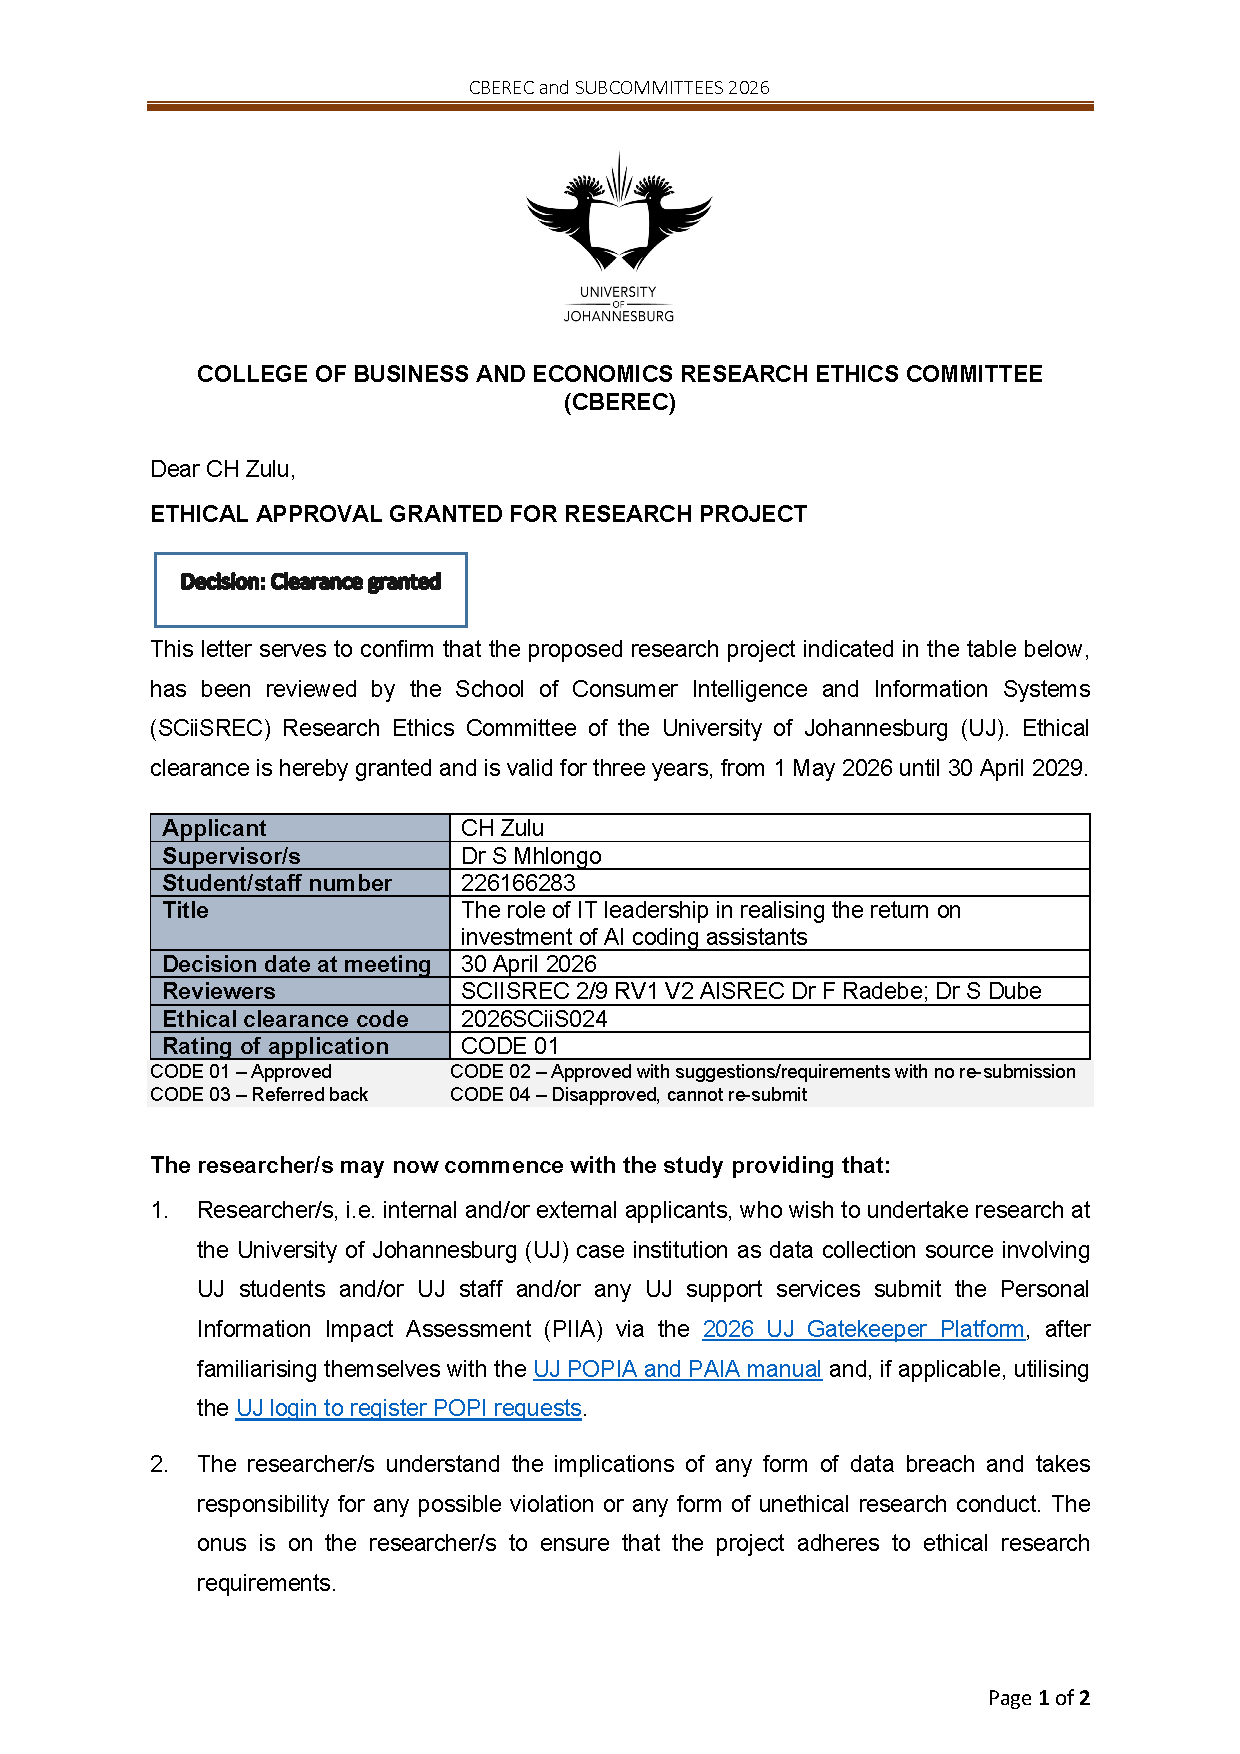
\includepdf[pages=-,scale=.9,pagecommand=\thispagestyle{fancy}]{PDF_Includes/7c_SCiiSREC_Ethical Clearance Report 2026SCiiS024_Zulu.pdf}

% ------------------------------------------------------------------------------
% Appendix Chapter: Sample Appendix Chapter
% ------------------------------------------------------------------------------
\chapter{Appendix Chapter}
\label{appendix:appendix_chapter}

\section{Appendix section}
\blindtext[1]

% ------------------------------------------------------------------------------
% Appendix Chapter: Sample Appendix Chapter
% ------------------------------------------------------------------------------
\chapter{Another Appendix Chapter}
\label{appendix:another_appendix_chapter}
\blindtext[1]
	
\end{document}